%%%%%%%%%%%%%%%%%%%%%%%%%%%%%%%%%%%%%%%%%%%%%%%%%%%%%%%%%%%%%%%%%%%%%%%%
\section{Language Modeling}
\label{sec:rw_lm}
%%%%%%%%%%%%%%%%%%%%%%%%%%%%%%%%%%%%%%%%%%%%%%%%%%%%%%%%%%%%%%%%%%%%%%%%


%%%%%%%%%%%%%%%%%%%%%%%%%%%%%%%%%%%%%%%%%%%%%%%%%%%%%%%%%%%%%%%%%%%%%%%%
\subsection{Introduction}
%%%%%%%%%%%%%%%%%%%%%%%%%%%%%%%%%%%%%%%%%%%%%%%%%%%%%%%%%%%%%%%%%%%%%%%%
A language model is a probabilistic model that predicts distributions over textual units conditioned on a context. Typically, these textual units will be subwords (or \textit{tokens}), noted as $(w_t)_{t\in[1, L]}$, and the language model (or \textit{LM}) predicts the following probability:
$$
P(w_T | w_{\neq T})
$$
where the context $w_{\neq T}$ is a subset of subwords taken from $(w_t)_{t\in[1, L] \setminus T}$.

These models can be used in various applications, which will often shape the way the context is built. For instance, for text generation purposes, the context will be a subset of textual units from the past that we can write as $w_{< T}$, as the model can only access text that has already been generated. Conversely, for a language correction system, it is possible to build language models that use every element of $(w_t)_{t\in[1, L] \setminus T}$ as the text already exists when the system is used.


%%%%%%%%%%%%%%%%%%%%%%%%%%%%%%%%%%%%%%%%%%%%%%%%%%%%%%%%%%%%%%%%%%%%%%%%
\subsection{Methods}

\paragraph*{Textual units and Tokenization}
\label{subsec:rw_lm_tokenization}

Before presenting the statistical paradigm of modern language models, we need to define precisely the textual units on which these models are based, namely tokens. \citet{mielke2021wordscharactersbriefhistory} cope with this subject in a very exhaustive manner. They distinguish three different approaches of forming tokens: a linguistic approach, an atomic approach, and a statistical approach.

First, many works have built linguistically-grounded sets of textual units that should be considered as microscopic to some extent, such as the Morphosyntactic Annotation Framework \citep{clement_maf}, which defines a token as a \textit{non-empty contiguous sequence of graphemes or phonemes in a document}. More generally, the domain of morphology, well defined in \citet{aronoff2022morphology}, has led to several morphologically-informed tokenizers \citep{saleva-lignos-2021-effectiveness, gronroos-etal-2018-cognate}.

The atomic approach takes a radically different stance. It consists in using shorter units, e.g. bytes, characters or pixels from a rendered text (see \Cref{sec:tokfree}). Although this choice seems less biased and restrictive than the latter, it immediately raises computational complexity concerns in LMs, as the necessary number of units can considerably increase.

Paying attention to the number of units used for a given text utterance logically leads to techniques that statistically optimize for this metric while keeping a meaningful segmentation scheme in order to maintain the feasibility of language modeling. 

\begin{figure}[h]
    \centering
    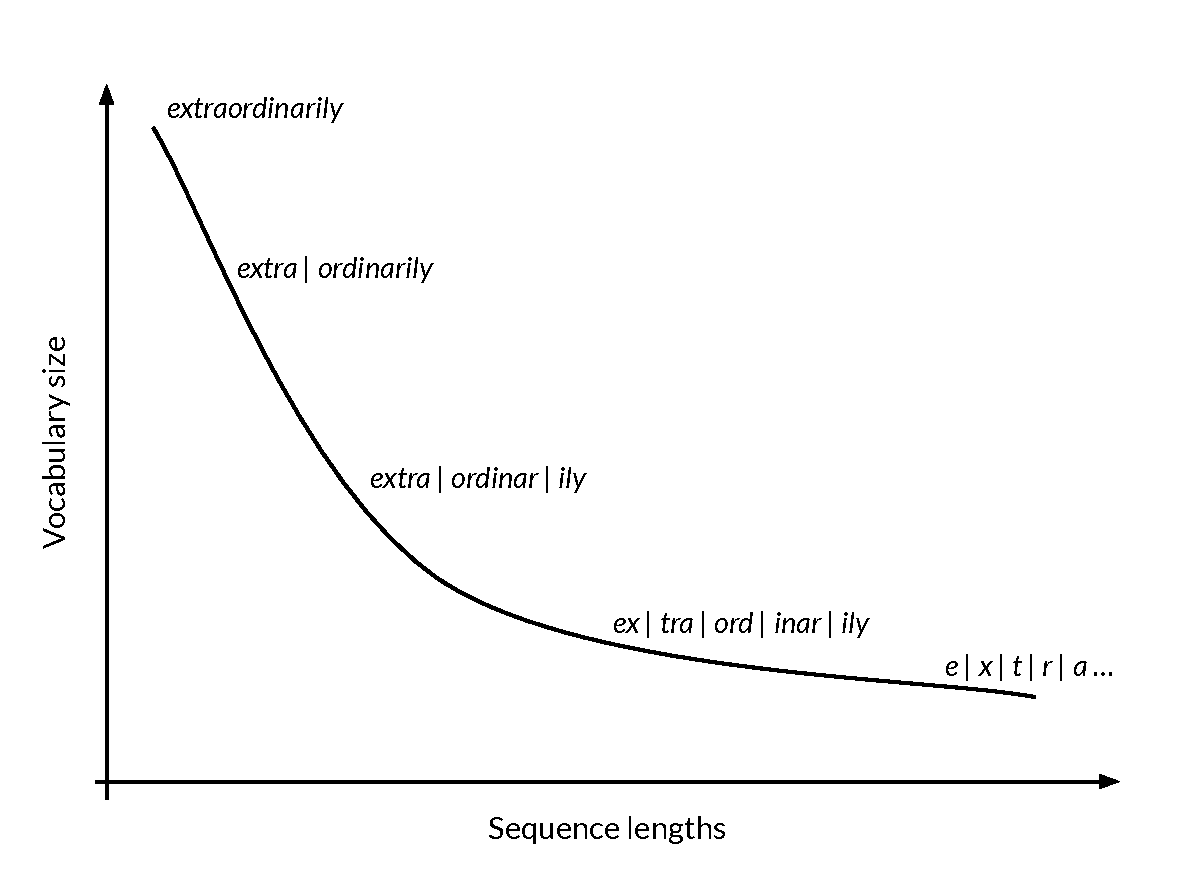
\includegraphics[width=0.5\linewidth]{sources/related_works/imgs/token_graph.pdf}
    \caption{}
    \label{fig:token_graph}
\end{figure}

Such statistical methods have dominated in the last few years as the default way to encode textual data, the most used being BPE \citep{sennrich-etal-2016-neural}, WordPiece \citep{wu2016google} and Unigram \citep{kudo-2018-subword}.

Byte-Pair Encoding, or BPE \citep{Gage1994bpe}, is a compression technique that relies on recursive symbol merges. In NLP, it is based on a dataset that consists in sequences of characters or bytes, and it iteratively registers a set of merge operations that reduce the count of merged items the most. WordPiece \citep{wu2016google} is based on a similar concept but uses a different rule for selecting merges. The possible merges $ab$ are scored according to:

$$
s(ab) = \frac{f_{ab}}{f_a \times f_b}
$$

where $f_{x}$ is the frequency of the string $x$ in the dataset. This scoring function differs from the basic BPE frequency as it favors merges $ab$ that appear in most cases when $a$ or $b$ appear. This typically leads to a more linguistically meaningful segmentation, as prefixes and suffixes are less prone to merging.

The Unigram tokenization algorithm \citep{kudo-2018-subword} works in the opposite direction : it first creates an exhaustive list of token candidates, and then iteratively removes tokens that affect the likelihood of the segmented sequence the least once discarded.

The statistical approaches are widely used in modern LMs, sometimes jointly with techniques such as subword regularization \citep{provilkov-etal-2020-bpe} that diversify segmentation results.

\paragraph*{Likelihood Maximization} Once the tokenization scheme is chosen, textual documents are parsed into sequences of tokens taken from a vocabulary of possible tokens  $\mathcal{V}$ of size $\left|\mathcal{V}\right| = V$. A \textit{training set} $T = (s_i)_{i\in[1, S]}$ of $S$ token sequences is thus built from the target textual documents. Each of these sequences $s_i$ has a given length $l_i$, and can also be written $s_i = (w_j)_{j \in [1, l_i]}$.

A language model $\phi_\theta$, based on a parameter set $\theta$, is a function that takes a sequence of tokens $\mathbf{w}_{\neq t}$ called context as an input, and outputs a probability distribution in $\Delta ^V$ for the token at position $t$.

The performance of a language model at token-level can be measured by computing the probability of the realization $w_t$ in the context $\mathbf{w}_{\neq t}$:
$$
\phi_\theta(\mathbf{w}_{\neq t})_{w_t} = P_\theta(w_t | \mathbf{w}_{\neq t})
$$

The process of training a language model consists in optimizing its average performance on the training set, which can be framed as a likelihood maximization objective \citep{mle}. In practice, to improve numerical stability, the objective is based on log-likelihood :
$$
\theta^* = \argmax_{\theta} E_T(\log \phi_\theta(\mathbf{w}_{\neq t})_{w_t})
$$

The minimized likelihood can also be seen as cross-entropy minimization between $P_\theta$ and an observed contextual probability distribution, estimated from the sample at position $t$, which is $\mathbf{1}_{w_t}$.

A metric that is often used to evaluate language modeling performance is \textit{perplexity} :
$$
\mathcal{P}(\phi_\theta, t) = 2^{-\log \phi_\theta(\mathbf{w}_{\neq t})_{w_t}}
$$


\subsection{Architectures}

\paragraph*{Statistical Methods}

The straightforward approach to language modeling consists in statistically estimating the distribution of tokens based on their context. 

In its most basic form, such statistical model estimates the \textit{unigram} distribution, that is the non-contextual distribution $P(w_t)$. This distribution is estimated by bin-counting tokens in the training dataset $T$ to retrieve token frequencies $f_w$ for each token $w$, and setting :
$$
\phi_{\theta}(\mathbf{w}_{\neq t}) = (f_w)_{w \in \mathcal{V}} \in \Delta^{V}
$$

We can extend this idea by estimating the \textit{2-gram} distribution $P(w_{t-1}w_t)$. To do so, we count the occurences of the subsequence $w_{-1} w_0$ in the training dataset for each pair of tokens $w_{-1}, w_0 \in \mathcal{V}^2$. Doing so, we can build a $V \times V$ stochastic matrix - i.e. which coefficients are non-negative reals that sum to $1$ column-wise - containing the observed frequencies for $w$ in pairs of the form $w_{-1} w$:
$$
M_2(T) = (f_{w_{-1} w})_{w_{-1}, w \in V^2}
$$
Then, the language model $\phi_{\theta}$ becomes:
$$
\phi_{\theta}(\mathbf{w}_{\neq t}) = (f_{w_{t-1} w})_{w \in V}
$$

More generally, $n$-gram language models \citep{jurafsky_course} can be designed to estimate the distribution $P(w_{t-n +1}...w_{t-1}w_t)$. By bin-counting $n$-uplet occurences in $T$, one can compute:
$$
M_n(T) = (f_{w_{-n+1}...w_{-1}w})_{(w_{-n+1}...w_{-1}), w \in V^{n-1} \times V}
$$
The associated language model $\phi_{\theta}$ can then be written:
$$
\phi_{\theta}(\mathbf{w}_{\neq t}) = (f_{w_{t-n+1}...w_{t-1} w})_{w \in V}
$$

These $n$-gram language models can be combined with backoff strategies to take sample size into accounts and switch between $n$ values when appropriate \citep{kneser_ney}.

\paragraph*{Neural Methods}
\citet{bengio2000neural} introduce the idea of training $\phi_\theta$ as a neural network with parameters $\theta$. The model is composed of three separate layers:

\begin{itemize}
    \item An \textbf{embedding} layer that corresponds to a look-up table that matches each token to a non-contextual feature vector that will be used as the input of the neural network;
    \item A hidden layer using a $\tanh$ non-linearity that maps the concatenation of $n$ input embeddings representing $w_{t-n+1}...w_{t-1}$ to an intermediate representation;
    \item An output layer that we call the \textbf{language modeling head} in reference to classification heads, that maps the intermediate representation to a $V$-dimensional vector.
\end{itemize}

\begin{figure}[h]
    \centering
    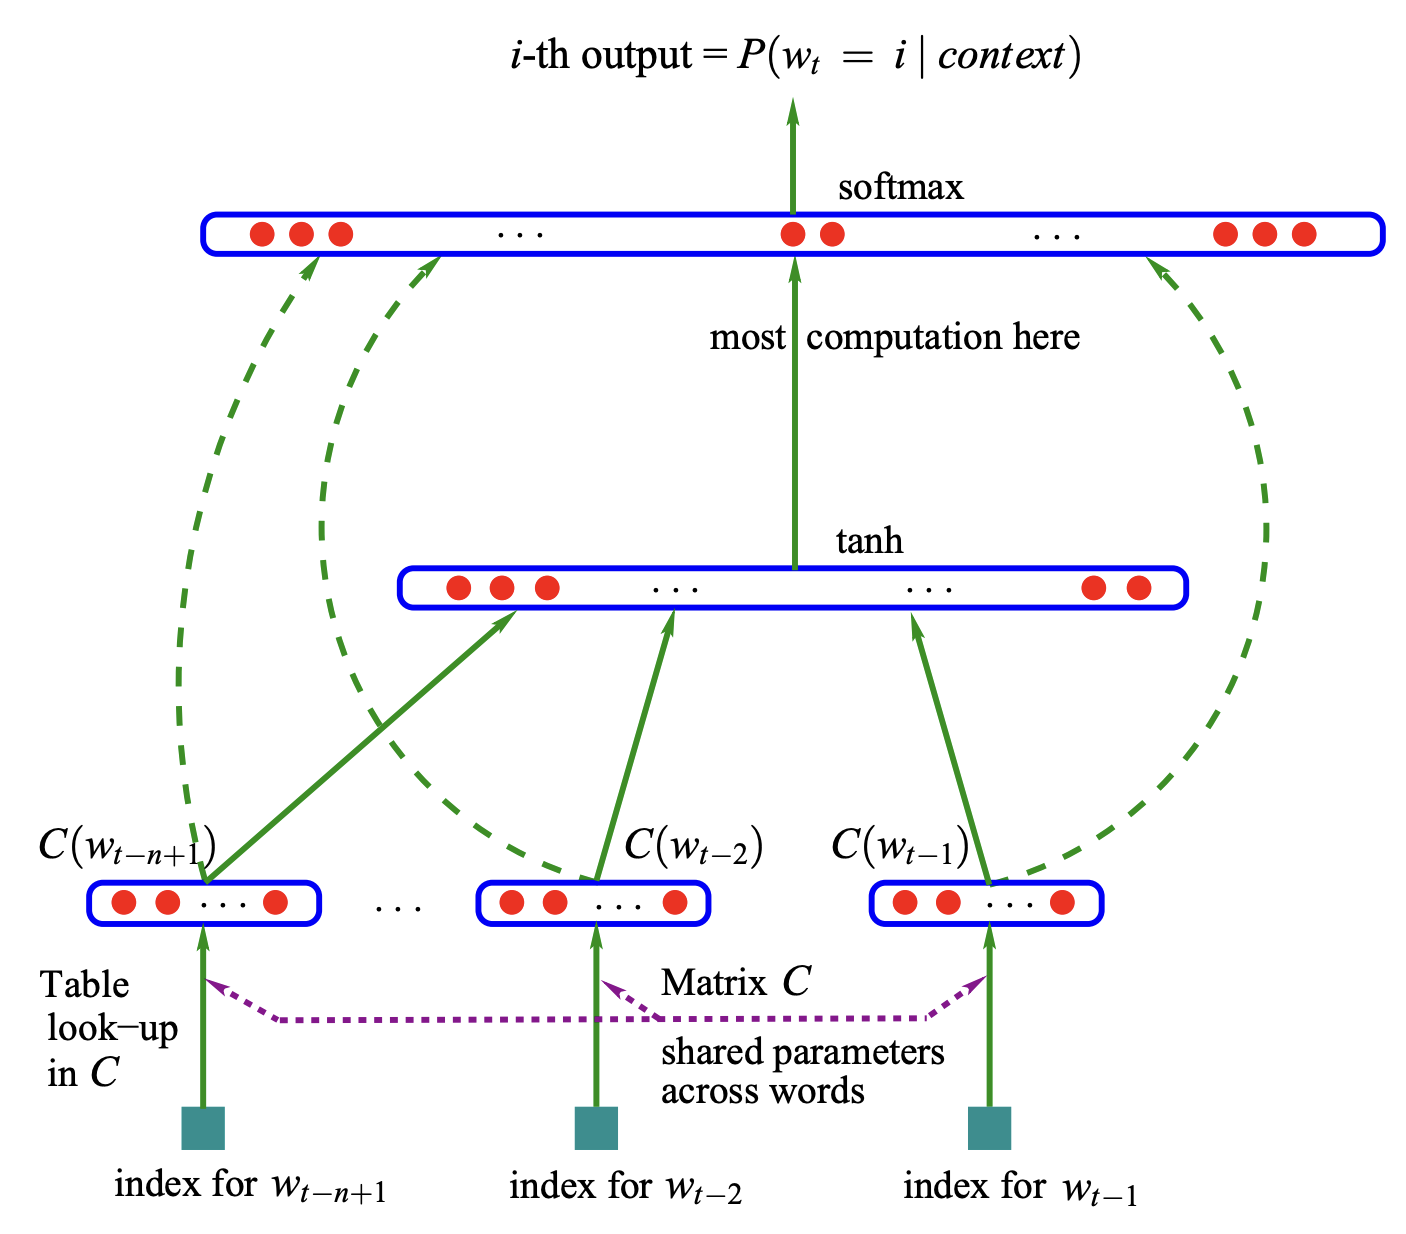
\includegraphics[width=0.5\linewidth]{sources/related_works/imgs/bengio_schema.png}
    \caption{Schema of a basic neural network architecture for language modeling (from \citet{bengio2000neural}).}
    \label{fig:bengio}
\end{figure}

The $V$-dimensional output is then normalized to a probability distribution using the softmax function. The softmax function $\zeta$ can be written component-wise for $x \in \mathbb{R}^d$ as :
$$
\zeta(x_i) = \frac{\exp(x_i)}{\sum_{j=1}^{d} \exp(x_j)}
$$

The model is then trained to optimize the log-likelihood using stochastic gradient descent (see \Cref{subsec:rl_optim}) on the parameters $\theta$ of the neural network.

\citet{bengio2000neural} train this neural architecture on the Brown corpus and the Associated Press News corpus and report substantial perplexity improvement compared with language models based on $n$-grams. This performance gap can be explained by the ability of neural networks to learn smooth contextual features, thus greatly improving extrapolation in the training feedback and at inference time.

A common trick that has been used in this framework is \textit{weight tying} \citep{press-wolf-2017-using}. It consists in using the same coefficients for the input embedding lookup table $W_{in} \in \mathbb{R}^{V \times d_m}$, and the language modeling head $W_{out} \in \mathbb{R}^{d_m \times V}$, by setting:
$$
W_{out} = W_{in}^T
$$
\citet{press-wolf-2017-using} show that this technique improves the performance of language models, while reducing their overall number of parameters.

\paragraph*{Recurrent Neural Networks}

A Recurrent Neural Networks (or \textit{RNN}) is a neural network that is trained to be applied sequentially to an input sequence, and that can use a past intermediate representation as input for present prediction. This concept was historically introduced in \citet{rnn_origins} but was first successfully applied to language modeling in \citet{mikolov10_interspeech}.

More precisely, input tokens are transformed into static embeddings using a similar look-up table as in \citet{bengio2000neural}, and a recurrent unit $\upsilon$ is then applied to the embedding sequence, sharing \textit{hidden states} $(h^1,...h^k)$ between each step of the sequential processing. The unit $\upsilon$ then processes the input embedding $x_t$ and the hidden states $(h_{t-1}^1,...h_{t-1}^k)$ at step $t$ through chosen tensor operations and non-linearities, returning an output representation $o_t$ in the process. The model can be described with this pattern:
$$
(o_{t}, (h_{t}^1,...h_{t}^k)) = \upsilon(x_t, (h_{t-1}^1,...h_{t-1}^k))
$$

Several variations have been proposed for this kind of models, notably improving the ability to avoid gradients issues related with the recurrence or to select information in the hidden states using specific functions in the unit. One of the most known variants is the Long Short-Term Memory (LSTM) unit introduced in \citet{HochSchm97} that has been widely used in NLP, including for language modeling \citep{miyamoto-cho-2016-gated}. The Gated Recurrent Unit (GRU) was later introduced in \citet{cho2014learningphraserepresentationsusing} as a simplification of the LSTM unit.

Although these units improve modeling abilities for long range dependencies \citep{rnn_eval}, they were empirically found to fail to handle interactions for elements separated by more than 1,000 time steps \citep{HochSchm97}.

\paragraph*{Transformers}

\citet{bahdanau_nmt} popularized the use of \textit{attention} in neural machine translation models as a method that lets the model select relevant tokens from the source sequence at a given prediction step. Such models, that previously used the last hidden states of a source-processing RNN (called \textit{encoder}) as the input to a target-generating RNN (called \textit{decoder}), suffered from an information bottleneck due to sharing only last-step representations between source and target sequences. The attention mechanism allowed to ease this bottleneck, by providing a \textit{direct path of interaction} between the source tokens and the decoder.

Attention was notably used in \citet{peters-etal-2018-deep} which use a bidirectional LSTM model for language modeling, before \textit{adapting} the model for downstream tasks, sometimes adding \textit{self-attention} layer (an attention mechanism that let a sequence interact with itself).

This idea was explored further in the notorious article \textit{Attention is All You Need} \citep{vaswani2017attention} that proposes to use attention as the only sequence-wise operation. As it is the main architecture that we will be using through our experiments, we proceed to thoroughly explain the inner workings of the Transformers block.

The original Transformers block or layer is a sequence processing block that mainly relies on Multi-Head Attention (or \textit{MHA}) to model inter-token interactions. The layer takes a sequence of $d_m$ dimensional representations $(x_t)_{t \in [1, L]}$ as an input, and outputs a similar sequence $(o_t)_{t \in [1, L]} \in \mathbb{R}^{L \times d_m}$. 

The input representations $x \in \mathbb{R}^{L \times d_m}$ are put through a multi-headed self-attention operation. More precisely, they are put through $3 \times n_h$ linear layers\footnote{For the sake of simplicity, we consider unbiased linear layers for the rest of this section.} with parameters $(W_Q^h, W_K^h, W_V^h)_{h \in [1, n_h]}$ of shape $d_m \times d_h$ where $n_h$ be the number of heads, and $d_h = \frac{d_m}{n_h}$. This constitutes three intermediate representations called queries $Q^h$, keys $K^h$, and values $V^h$ of shape $L \times d_h$:
\begin{equation*}
    \begin{cases}
        Q^h = x W_Q^h \\
        K^h = x W_K^h \\
        V^h = x W_V^h
    \end{cases}
\end{equation*}

Queries and keys are used to determine interaction weights between input representations via an attention map $A^h$ of shape $L \times L$, that is computed as:
$$
A^h = \text{softmax} \left(\frac{Q^h {K^h}^T}{\sqrt{d_h}}\right)
$$

The head-level output representations $v^h$ of shape $L \times d_h$ can then be understood as weighted sums of values based on the attention map rows:

$$
v^h = A^h V^h
$$

Finally, head-level representations are concatenated into the output representations of shape $L \times d_m$ and projected using a $d_m \times d_m$ linear layer of weights $W_o$:

$$
o = \text{concatenate}_{h\in [1, n_h]}(v^h) W_o
$$

This self-attention layer can be summarized in the following formula:
\begin{equation}
    \label{eq:self_attn}
o = \text{concatenate}_{h\in [1, n_h]} \left( \text{softmax} \left(\frac{x W_Q^h {W_K^h}^T x^T}{\sqrt{d_h}}\right) x W_V^h \right) W_o
\end{equation}


The authors argue that the main modeling improvement that this architecture yields is the direct cross-representation interactions that are allowed by the $Q^h {K^h}^T$ product, compared to the indirect interactions that are modeled in RNNs. Indeed, this matrix product can be decomposed into scalar products between queries and keys from different positions $i$ and $j$ in the sequence:

$$
(Q^h {K^h}^T)_{i, j} = \langle Q^h_i , K^h_j \rangle
$$

However, this modeling advantage comes at a quadratic cost in memory and time complexity, as the attention map needs to be computed using $O(L^2)$ operations, and stored using $O(L^2)$ floats. Variants propose to tackle this quadratic cost by restricting the $(i, j)$ position pairs where attention is computed, or by reducing the attention map size using various methods (see \Cref{subsec:efficient_attn}).

The expression of self-attention in \Cref{eq:self_attn} is non-causal, i.e. the output representation $o_t$ is a result of operations that can use input representations $x_t, x_{t+1}, ..., x_L$. For causal language modeling, where the used context should be $\mathbf{w}_{< t}$, the $o_t$ representation cannot be used for prediction at index $t + 1$ as it carries information from the future of the sequence, including $w_{t+1}$ through $x_{t+1}$. Hence, this architecture is not suited for a causal language model (or CLM) as such.

To account for causality in the self-attention operation, we can introduce a \textit{causal mask} $\mathcal{M}$ that will null out every non-causal interaction in the attention map, thus leading to $A^h_{ij} = 0$ when $i > j$. To do so, we instantiate $\mathcal{M}$ as:
\begin{equation*}
    \mathcal{M} = \begin{pmatrix}
        0 & -\infty & \cdots & -\infty \\
        \vdots & \ddots & \ddots & \vdots \\
        \vdots &  & \ddots & -\infty \\
        0 & \cdots & \cdots & 0

    \end{pmatrix}
\end{equation*}

We can then compute a causal self-attention map $A^h$ as:
$$
A^h = \text{softmax} \left(\frac{Q^h {K^h}^T}{\sqrt{d_h}} + \mathcal{M} \right)
$$

Now, $o_t$ only has access to representations $\mathbf{x}_{<t+1}$, and can directly be used for prediction at position $t+1$.

However, the Transformers block does not use the outputs of the self-attention operation directly, but rather surrounds the self-attention operation with highly-parameterized linear layers and normalizations. 

The representations $o$ are first summed with $x$ through a residual connection, which eases optimization and stabilizes gradients \citep{residual_conn}. The output is then regularized using layer normalization \citep{ba2016layernormalization}. Layer normalization is a form of representation regularization that avoids gradient-related issues due to the accumulation of layers. For a given set of representations $(e_t)_{t\in [1, L]}$, it performs the following normalization:
$$
\text{LayerNorm}(e_t)_i = \frac{e_{t, i} - \bar{e_t}}{\sqrt{\frac{1}{L} \sum_{j=1}^{L} (e_{t, j} - \bar{e_t})^2}} \times \gamma_i + \beta_i
$$

where $\bar{e_t}=\frac{1}{L} \sum_{j=1}^{L} e_{t, j}$ and $\gamma$ and $\beta$ are network parameters.

The Transformers block is then composed of a \textit{feed-forward} block, which is itself made of an upscaling linear layer of weights $W_{up} \in \mathbb{R}^{d_m \times d_{up}}$, an activation function and a downscaling linear layer of weights $W_{down} \in \mathbb{R}^{d_{up} \times d_m}$. A common choice for $d_{up}$ is $4 \cdot d_m$, and the activation function is typically one of ReLU \citep{relu}, GELU \citep{hendrycks2023gaussianerrorlinearunits} or SiLU \citep{silu}.

The last part of the block consists of another residual connection that adds the output of the first layer normalization to the output of the feed-forward layer, followed by a final layer normalization.

A Transformers model consists in a stack of Transformers block followed by a language modeling head of shape $d_m \times V$ that outputs logits $(l_t)_{t \in [1, L]}$. The Transformers causal language model $\phi_\theta$ for $t \in [2, L+1]$ can thus be written:

$$
\phi_\theta(\mathbf{w}_{<t}) = \text{softmax} (l_{t-1})
$$

Such a Transformers model based on causal self-attention is usually refered to as a decoder model, as it can be used as a decoder in a sequence-to-sequence model, in Machine Translation for instance. When causality does not matter for the targeted task, self-attention can be computed without the causality mask $\mathcal{M}$, which leads to an \textit{encoder} architecture.

In \citet{vaswani2017attention}, the main task is Neural Machine Translation, which leads to the use of an \textit{encoder-decoder} architecture. The source sequence is processed through an encoder Transformers, and the target sequence logits are generated using causal self-attention blocks with an added cross-attention layer. Cross-attention is similar to self-attention, but uses $Q^h$ and $K^h$ representations from one sequence and $V^h$ from another sequence. In the terms of \Cref{eq:self_attn}, cross-attention between sequences $x$ and $y$ can be written:

\begin{equation}
    \label{eq:causal_attn}
o = \text{concatenate}_{h\in [1, n_h]} \left( \text{softmax} \left(\frac{x W_Q^h {W_K^h}^T x^T}{\sqrt{d_h}}\right) y W_V^h \right) W_o
\end{equation}

A substantial difference between RNNs and Transformers is that positional information is not encoded naturally in the intermediate representations. Hence, several approaches have been introduced to embed positional information in Transformers models. These approaches can be split into two families: absolute positial embeddings (APE) and relative positional embeddings (RPE).

Absolute positional embeddings encode the position corresponding to the index of an item in the processed sequence. In \citet{vaswani2017attention}, the authors use sinusoidal functions to build representations of shape $d_m$ and add them to the input embeddings of the model. However, after \citet{devlin-etal-2019-bert}, the main approach has been to create a $L \times d_m$ lookup table of learnable parameters, and use row $i$ as a positional embedding for position $i$. The main limitation of such positional embeddings is that a model trained on sequences of length $L$ will be unable to process sequences of length longer than $L$, as no positional embeddings will be available for the additional positions.

Relative positional embeddings encode pairwise positional information in the self-attention map $A_h$ directly, and more specifically to the $Q^h {K^h}^T$ product. Usually, for a position pair $i, j$, RPE define functions $\omega_i$ and $\omega_j$, and a bias term $\beta_{ij}$:
\begin{equation}
    \label{eq:rpe}
(Q^h {K^h}^T)_{ij} = \langle \omega_i(Q^h_i), \omega_j(Q^h_j) \rangle + \beta_{ij}
\end{equation}

The most used RPE approaches are Rotary Positional Embeddings or RoPE \citep{rope}, and Attention with Linear Biases or ALiBi \citep{alibi}. In the framework of \Cref{eq:rpe}, RoPE can be expressed as:
$$
\begin{cases}
    \omega_i(x) = \mathbf{R^{d_m}_i}x \\
    \beta_{ij} = 0
\end{cases}
$$
where $\mathbf{R^{d_m}_i}$ is a rotary matrix that rotates pairs of dimensions with different angles depending on $i$. It can be written as the following blockwise diagonal matrix:
$$
\mathbf{R^{d_m}_i} = \begin{pmatrix}
    R_{i, \theta_1} & 0 & \cdots & 0 \\
    0 & \ddots & \ddots & \vdots \\
    \vdots & \ddots & \ddots & 0 \\
    0 & \cdots & 0 &  R_{i, \theta_{d_m/2}} \\
\end{pmatrix}
$$

where $R_{i, \theta} = \begin{pmatrix}
    \cos i \theta & -\sin i \theta \\
    \sin i \theta & \cos i \theta
\end{pmatrix}$ and $\theta_d = 10000^{\frac{-2(d-1)}{d_m}}$.

\citet{alibi} use a more straightforward approach. Their RPE, which relies on a linear bias on the whole attention map, can be written:
$$
\begin{cases}
    \omega_i(x) = x \\
    \beta_{ij} = m (i-j)
\end{cases}
$$
with $m \in \mathbb{R}$ as a head-specific fixed parameter.

\paragraph{Generation \& KV Cache}

Causal language models can be used for natural language generation, by sampling from the next-token probability and iterating over the sampled token or tokens. Although various generation strategies exist \citep{fan-etal-2018-hierarchical, wang2020contextual, nucleus_sampling}, the most straightforward one is greedy sampling, where the highest-probability next token is chosen and added to the generated sequence iteratively:
$$
w_{t+1} = \argmax_{w \in \mathcal{V}}\phi_{\theta}(\mathbf{w}_{<t+1})_w
$$

For RNNs, language generation is rather straightforward as the unit just requires the last hidden state and the current token input representation to make a prediction. For Transformers models however, a naive approach could consist in applying the model to the whole past sequence at each generation step, which would be $O(L^3)$ in time complexity. Luckily, the causal masking in self-attention implies that the post-attention representations $o$, which just depend on their own past, would be constant over generation steps, except for the last one $o_t$.

Hence, it is possible to cache the representations with indexes $i < t$ needed to generate $o_t$, which are $(K^h_i)_{i<t}$ and $(V^h_i)_{i<t}$. This caching technique is named KV caching.

\paragraph{Trained Models and Variants}
Highly influential Transformer-based language modeling works led to different model families : GPT \citep{Radford2018ImprovingLU}, BERT \citep{devlin-etal-2019-bert} and T5 \citep{2020t5}.

GPT (for \textit{Generative Pre-trained Transformer}) is a Transformers-based architecture that trains a decoder model for causal language modeling in a straightforward way. The training set is BookCorpus \citep{bookcorpus}, which contains unpublished books from a variety of genres. The authors use a 12-layer decoder-only Transformer with $d_m=768$, $n_h=12$ attention heads and a vocabulary of $V=40000$ tokens. Overall, GPT counts 110 million parameters.

GPT is used as a pre-trained model, and is thus fine-tuned for Natural Language Understanding downstream tasks from the GLUE benchmark \citep{wang-etal-2018-glue}. These tasks being mostly sentence-level classification tasks, the language modeling head of GPT is thus replaced with a pooling layer that extract a single representation from the output embeddings sequence by averaging or retaining the maximal value across hidden dimensions, followed by a classification head of shape $d_m \times n_c$ where $n_c$ is the number of classes for the target downstream task.

BERT (for \textit{Bidirectional Encoder Representations from Transformers}) is an encoder-only architecture trained for Masked Language Modeling or \textit{MLM}. A masked language model is a language model that uses the full context $\mathbf{w}_{\neq t}$ for the prediction at index $t$, which is called the masked token. In BERT, the authors propose to alter input token $w_t$ in the following way:
\begin{itemize}
    \item Replace it with a specific mask token 80\% of the time;
    \item Replace it with a random token 10\% of the time;
    \item Leave it unchanged 10\% of the time.\footnote{In that case, the training task is not language modeling but simply learning the identity mapping.}
\end{itemize}

In \citet{devlin-etal-2019-bert}, 15\% of the tokens are masked according to this procedure, and the cross-entropy training objective is used for the masked positions. By partially masking the whole sequence at once, the authors assume that altering one token does not hurt the feasability of the prediction at another position which uses this token in the context. In order to train the model for sentence-level semantics, an auxiliary objective trains the model to identify whether two consecutive sentences in the training data were also consecutive in the original document.
The original trained architecture is similar to GPT in parameter count and is similarly fine-tuned on downstream tasks, but a larger version is trained and achieves better performance. \citet{roberta} subsequently show that training on larger training sets leads to significantly better performance, and introduce the RoBERTa models suite.

T5 (for \textit{Text-to-Text Transfer Transformer}) is a model suite that aims for a different approach when it comes to downstream tasks. \citet{2020t5} argue that downstream tasks can be rephrased as natural language samples. For instance, the Corpus of Linguistic Acceptability, or CoLA \citep{warstadt2018neural} is a sentence-level classification task where a grammatical acceptability label (acceptable or unacceptable) is given to each sentence. The STSB subset of GLUE \citep{wang-etal-2018-glue} is a sentence-pair classification task where a similarity score in $[1, 5]$ is given to a pair of sentences. The authors argue that these tasks can be rephrased as language modeling tasks where the labels or scores are tokens that the model is expected to generate at inference time. The main advantage of this approach is that it does not require to have task-specific classification heads, which implies that the model can be fine-tuned on all tasks at once.

An optimized architecture for this task should be able to process an input sequence bidirectionally, and to generate a label for this input sequence. Thus, a natural choice is an encoder-decoder architecture, where the input sequence will be processed using the non-causal encoder, and a decoder using causal self-attention and cross-attention to the encoded sequence to generate the target label. \citet{2020t5} pretrain an encoder-decoder architecture for the language in-filling task, which extracts contiguous spans of tokens in the sequence, and trains a causal language model on these spans, using the rest of the sequence as the context. More formally, if the extracted span is $t_0, ..., t_0+\eta$, the T5 objective trains a causal language model on tokens $(w_i)_{i \in [t_0, t_0+\eta]}$ using context:
$$
\mathbf{w}_{\neq t} = (w_i)_{i \in [1, t] \cup ]t_0+\eta, L]}
$$

In T5, similarly to BERT, several spans are masked at once to avoid reprocessing the sequence, and under the assumption that it would maintain sufficient information to make convincing predictions. The authors release several models ranging from 60 million to 11 billion parameters for English language.

Following these works that mostly focus on English, several multilingual counterparts were released. Notable examples include mBERT, XLM-RoBERTa \citep{conneau2019unsupervised}, mGPT \citep{mgpt} or mT5 \citep{xue-etal-2021-mt5}.

\citet{electra} later notice that both GPT-like and BERT-like approaches are suboptimal when it comes to learning fine-tunable contextual representations using self-supervised methods. As a matter of fact, the contextual representations extracted from causal language models do not contain bidirectional information. On the other hand, only a fraction of the tokens are directly used when training masked language models, which may harm the data and compute efficiency of such an approach. \citet{electra} combine both these strenghts into the ELECTRA scheme: their pretraining approach directly uses every token available in each mini-batch, but also allows non-causal self-attention in the trained models. To that end, they use \textit{Replaced Token Detection} as a self-supervised task. They train two models: a smaller masked language model called the \textit{generator}, and a larger Transformers architecture called the \textit{discriminator}.

As in BERT \citep{devlin-etal-2019-bert}, a portion of the tokens is selected and used to pretrain the generator. The token associated with the highest predicted probability is then inserted at the selected position, and the resulting sequence is given as an input to the larger discriminator. The discriminator outputs a single float in $[0, 1]$ for each input token, which is trained to predict the probability that a position corresponds to a \textit{replaced} token, ie. a token that has been modified by the generator.

They conduct medium-scale experiments, training models ranging from 14M to 335M parameters, and observe that their pretrained models achieve parity with CLMs and MLMs when fine-tuned on downstream tasks, while using significantly less pretraining compute.


\paragraph*{Scale \& Performance}
The emergence of highly parameterized neural networks trained on large textual datasets as effective language models brings the question of scale, i.e. to what extent can scaling up either (or both) the volume of textual data or the count of trainable parameters can increase the language modeling performance and the downstream capabilities of models?

With RoBERTa \citep{roberta}, it appeared clear that the first generation of pretrained models, namely BERT and GPT, were undertrained. The authors train a BERT-style model on approximately 10 times more data, and remove the sentence-level auxiliary objective and show strong improvements. GPT-2 \citep{gpt2} is a follow-up model suite that was trained on a larger and more diverse dataset than BookCorpus called WebText, with model sizes ranging from 117 million to 1.5 billion parameters. The authors noticed that the larger GPT-2 models had interestingly better \textit{few-shot} and \textit{zero-shot} abilities, especially at question answering tasks.

GPT-3 \citep{gpt3} introduces a much larger architecture, using 175 billion parameters, while relying on a training procedure and architecture that do not significantly differ from the original Transformers-based GPT. The authors claim that this model displays a zero-shot downstream performance level that is close to fine-tuned counterparts. Similar results are reproduced through the OPT initiative \citep{zhang2022opt}. Subsequently, the 540 billion parameters PaLM model \citep{palm} was released, leading to similar conclusions. A multilingual counterpart to this line of work is BLOOM \citep{le2023bloom}, a 176 billion parameters model trained in 46 languages.

However well these models may perform, their training and inference raise a number of issues. Training these models consumes significant amounts of computational power, as it usually implies running thousands of Graphical Processing Units (GPUs) for multiple days, weeks or months. Moreover, these models are trained on enormous amounts of web-scraped textual data, which incentivizes the preparation of massive automatically cleaned textual datasets such as OSCAR \citep{oscar}, The Pile \citep{gao2020pile} or RedPajama \citep{together2023redpajama}. These datasets contain up to several trillions of tokens, which stands as a hard ceiling for language model training. Hence, it is both unclear whether it will be possible to train substantially larger language models on substantially larger text datasets, raising concerns about the possibility of a straightforward upscaling approach as a way forward for language modeling.

From the first Transformers-based models, the question of training optimal LMs under computational constraint has been considered in various ways. \citet{sanh2019distilbert} use knowledge distillation, i.e. using logits from a larger model as an objective for a smaller one, to train a smaller alternative to the base version of BERT that maintains a solid level of performance at reduced training and inference costs. \citet{turc2019} train a large set of small masked language models and show that pretraining student models before distillation leads to better performance. Other approaches have explored variants of knowledge distillation to improve performance for smaller models \citep{Fu_Zhou_Yang_Tang_Liu_Liu_Li_2021,sun-etal-2020-contrastive}.

A crucial result regarding the question of scaling is the empirical identification of \textit{scaling laws}, i.e. of explicit forms that accurately predict the final performance of a Transformers-based model based on $N$ non-embedding parameters and trained with a dataset composed of $D$ tokens. \citet{kaplan_scaling} are the first to discover this phenomenon, and they identify a scaling law that predicts the final cross-entropy loss $L(N, D)$ :
\begin{equation}
    \label{eq:kaplan}
L(N, D) = \left( \left(\frac{N_c}{N}\right)^{\frac{\alpha_N}{\alpha_D}} + \frac{D_c}{D}\right)^{\alpha_D}
\end{equation}
where $\alpha_N \approx 0.076$, $N_c \approx 8.8 \times 10^{13}$, $\alpha_D \approx 0.095$ and $D_c \approx 5.4 \times 10^{13}$ are empirically estimated parameters. \Cref{eq:kaplan} unsurprisingly predicts that LMs using more parameters or larger training datasets should have better language modeling performance. Moreover, it interestingly shows that for a fixed compute level $C \approx 6 N \cdot D$, there exist $N^*(C)$ and $D^*(C)$ that minimize $L$, so that training a larger model on less tokens or training a smaller model on more tokens both lead to poorer performance. Empirically, the values of $N^*(C)$ and $D^*(C)$ imply that the compute-optimal approach to language modeling consists in training relatively large models on small amounts of tokens.

However, \citet{chinchilla_scaling} suggest that the empirical results from \citet{kaplan_scaling} were not accurate. They first notice that \citet{kaplan_scaling} used intermediate checkpoints taken before complete cooldown, implying underestimated low-data performance. They also underline that there is a slight curvature of the scaling law by exploring larger model sizes to interpolate their scaling law. Their scaling law can be written:
\begin{equation}
    \label{eq:chinchilla}
    L(N, D) = \frac{A}{N^\alpha} + \frac{B}{D^\beta} + E
\end{equation}
where $A=406.4$, $B=410.7$, $\beta=0.28$, $\alpha=0.34$ and $E=1.69$.

Although the predicted pattern still implies that more parameters and/or training tokens lead to better log-likelihood levels, the values of $N^*(C)$ and $D^*(C)$ are leaning towards smaller models and larger amounts of tokens compared to \citet{kaplan_scaling}. Another notable difference is the introduction of a strictly positive limit to the loss when $N \rightarrow \infty$ and $D \rightarrow \infty$, which can be interpreted as the residual entropy of English language.

The scaling laws yield optimal $N$ and $D$ values for a fixed total training compute level $C$. However, they do not include inference computation cost in their equations, while it grows as the model size $N$ increases. \citet{beyond_chinchilla} take inference cost into account using \Cref{eq:chinchilla} and thus incentivize the training of even smaller models on larger datasets. Recent initiatives \citep{tinyllama,faysse2024croissantllm,gemmateam2024gemma} have followed this principle.

\subsection{Limitations \& Extensions}

\paragraph{The Softmax Bottleneck}

The concept of \textit{softmax bottleneck} was introduced in \citet{softmax_bottleneck}. In this article, the authors view the language modeling task through a matrix factorization prism. They decompose the language model $\phi_\theta$ into two parts : a model that outputs contextual embeddings $h_\theta(\mathbf{w}_{\neq t})$ of shape $d_m$, and a language modeling head $W_\theta \in \mathbb{R}^{d_m \times V}$:
$$
\phi_\theta(\mathbf{w}_{\neq t}) = \sigma (h_\theta(\mathbf{w}_{\neq t}) W_\theta)
$$

In a finite-length sequence framework, where possible contexts $\mathbf{w}_{\neq t}$ are countable, a contextual probability matrix can also be defined from the true distribution $P(w | \mathbf{w}_{\neq t})$:
$$
A = (\log P(w_i | c_j))_{i \in [1, V], j \in [1, C]}
$$
where $(c_j)_{j\in [1, C]}$ are the $C$ possible contexts.
Similarly, the language model can be described by the matrix:
$$
A_\theta = (\phi_\theta(c_j)_i)_{i \in [1, V], j \in [1, C]}
$$ 

The authors show that when $\rank A_\theta < \rank A$, which is likely when $d_m \ll V$, there exists contexts where the contextual probability distribution from $\phi_\theta$ cannot match the true distribution $P$.

They proceed to argue that $\rank A$ should be very high for natural language. In practice, measuring $\rank A$ would imply getting access to $A$ which is impossible. However, it can be argue that the distribution of tokens is highly context-dependent, as one single token (e.g. a negation marker) can imply a complete shift in token distribution at later positions. It is also unlikely that $\rank A$ is low as it does not seem plausible that only a few hundred of bases can express the whole diversity of contexts in language. These arguments hint towards higher rank values for $A$.

They propose to increase the possible rank of the language modeling head using a Mixture-of-Softmax. The language model is now decomposed into a first part that outputs $K$ contextual representations $h^k_\theta(\mathbf{w}_{\neq t})$ and a predicted mixture distribution $\pi_\theta(\mathbf{w}_{\neq t}) \in \Delta^K$ itself computed from hidden states through a softmax activation. The language model is then written:
$$
\phi_\theta(\mathbf{w}_{\neq t}) = \sum_{k=1}^K \pi_\theta(\mathbf{w}_{\neq t})_k \cdot \sigma (h^k_\theta(\mathbf{w}_{\neq t}) W_\theta)
$$

They argue that this Mixture-of-Softmax is more expressive that the vanilla approach, and provide experimental results in this direction.

Subsequent works have further explored the limitations of the softmax linear layer on language modeling performance, especially  \citep{chang-mccallum-2022-softmax} and other possible alternatives that rely on replacing the softmax layer with a more expressive counterpart \citep{lin2021breaking,sigsoftmax}. \citet{grivas-etal-2022-low} show that low-rank softmax layers can even lead to tokens that, although appearing in the training data, are never being predicted as the top-probability picks, and are thus never generated through greedy sampling.

\paragraph*{Tokenization}

Some of the induced biases of tokenizers can be harmful for modelization. One such limitation lies in their brittleness to character deformations which are commonly found in real world, noisy data. For instance, BERT's tokenizer~\cite{devlin-etal-2019-bert} encodes ``performance'' as \texttt{[``performance'']} but \mbox{``perfonmance''} as \texttt{[`per', `\#\#fo', `\#\#n', `\#\#man', `\#\#ce']}, which makes it hard for the model to behave similarly in both cases. Moreover, the tokenizer is fixed after its training and is therefore impossible to update without retraining, for instance to reflect new domains~\cite{el-boukkouri-etal-2020-characterbert} where tokenization might over-segment specific or technical terms. \citet{clark2022canine} list other issues emerging when using static subword tokenizers, especially when modeling languages with a more complex morphology than English.

Tokenizers are also a limitation when it comes to multilingual models. \citet{rust-etal-2021-good} show that training models using monolingual tokenizers systematically leads to better performance compared with multilingual ones. \citet{NEURIPS2023_74bb24dc} show that a single sentence can be 15 times shorter than its translation in another language. Moreover, the use of multilingual tokenizers often leads to the use of larger vocabularies which results in more weights being assigned to input embeddings. Nevertheless, \citet{liang2023xlmv} show that larger vocabularies lead to better downstream performance, thus indicating that multilingual models should ideally be able to handle such vocabularies at reduced cost.

\paragraph*{Character-level Models} Several alternative methods have been proposed to mitigate these tokenization issues.
This line-of-work suggests to learn character-level or byte-level representation for LMs instead of subword-level ones. These methods improve the robustness of LMs to naturally occurring noise as well as their expressiveness when dealing with out-of-domain or multilingual data. In order to cope with increased input lengths, some of these methods compress sequences with constant reduction rates obtained using specialized modules~\cite{clark2022canine,tay2021charformer}, subsequently removing any notion of subwords.

Some of the first neural networks for sequence generation used characters directly as inputs \citep{sutskever2011generating,graves2013generating}, and following works modified the approach to create input word representations based on characters \citep{kim2016character,Jzefowicz2016ExploringTL,peters-etal-2018-deep}. Similar architectures were recently adapted to work with Transformers. Notably, CharacterBERT \citep{el-boukkouri-etal-2020-characterbert} constructs whole word representations from character embeddings put through convolutions and highway layers, before feeding them to a Transformers architecture. \citet{ma-etal-2020-charbert} take this idea further by learning a BERT-style language model at character-level without intermediate pooling. 

Nevertheless, they still rely on fixed tokenization heuristics (for instance segmenting using whitespaces) which may not be suited to some languages or certain types of language variations. Several works have tried to remove these induced biases by working purely with characters or bytes as input. CANINE \citep{clark-etal-2022-canine} downsamples contextualized character representations via a strided convolution before feeding them to a Transformers. It can be trained either with a subword-based objective (CANINE-s) or with a character-level one (CANINE-c). \citet{tay2021charformer} design a similar model by replacing convolutions with efficient Transformers \citep{beltagy2020longformer}. A more direct approach, ByT5 \citep{xue-etal-2022-byt5} is a version of T5 that is trained at byte-level. Finally, \citet{yu2023megabyte} introduce the MEGABYTE model, by using a basic strided pooling approach to apply a Transformer architecture on $4$-bytes representations before using a more efficient model to decode these representations back to byte-level.

However, these methods either have to use various tricks to reduce the sequence lengths based on other induced biases like downsampling rates or have extremely low training and inference speeds \citep{xue2022byt5}. \citet{chung2016hierarchical} create tokens in a differentiable manner by predicting frontiers and using the representations of each character inside a ``token'', but it remains unclear how their model could be adapted to be used with newer architectures such as Transformers. \citet{mofijul2022vocabulary} propose to segment tokens using a trained ``frontier predictor.'' Nevertheless, this differentiable tokenizer is not trained with the main language model objective but instead mimics a BPE subword tokenizer, carrying some of its flaws.

Concurrently to this work, \citet{nawrot-etal-2023-efficient} propose to learn a dynamic tokenization scheme, using a module that predicts frontier positions and pools input bytes accordingly. They notably propose to use Gumbel noise \citep{gumbel-orig} through a sigmoid activation to sample a frontier decision variable in a differentiable manner. They proceed to train a differentiable tokenization scheme and succesfully reduce the perplexity and the latency of the language models on various languages.


\paragraph*{Efficient Self-Attention}

Self-attention has a quadratic complexity with respect to the sequence length $L$, as it requires the whole attention map $A \in \mathbb{R}^{L \times L}$ to be computed. In order to accelerate Transformers-based models, especially in long-context situations, several works have considered computing a subset only of the inter-positional interactions, or compressed versions of $A$. 

Notably, \citet{beltagy2020longformer} propose several alternatives in their Longformer architecture. First, they suggest only computing coefficients $(i, j)$ where $|i - j| < \delta$, thus resulting in a \textit{sliding window} pattern which gives its name to the method later used in Mistral models \citep{jiang2023mistral}. They proceed to present two variations of the sliding window attention: the first relies on a dilated pattern, and the second one allows a portion of the positions to use global attention, that is for a portion of $i$ values, the attention map value is computed at all positions $(i, j)$ for $j \in [1, L]$. These alternatives naturally come with their causal counterpart, for which the non-causal interactions are not included in the targeted  $(i, j)$ positions. The Longformer attention maps can be computed in $O(\delta L)$, which greatly accelerates inference in training when $\delta \ll L$.

The Linformer architecture \citep{wang2020linformer} takes a different direction and rather compresses $K^h$ and $V^h$ representations of shape $L \times d_h$ into representations of shape $k \times d_h$ using two $L \times k$ linear layers where $k \ll L$. The complexity of computing the self-attention maps becomes $O(k^2)$, allowing substantial acceleration at training and inference time. Similarly, \citet{nystromformer} use a Nyström decomposition of the attention map and achieve $O(L)$ complexity.

\paragraph*{KV Cache Compression}

As larger open-sourced models trained by industrial institutions emerged \citep{jiang2023mistral,touvron2023llama}, many efforts have aimed at improving the efficiency of self-attention as a \textit{post-training} step. This novel incentive paved the way for algorithms designed specifically for optimizing the attention maps of trained models. These algorithms usually avoid editing parameters of the model and are instead framed as \textit{KV cache compression}, as they indeed compress the cached $K^h$ and $V^h$ representations under language modeling performance constraints.

During generation, the KV cache grows linearly in size and it represents a total of :
$$
|KV|(t) = 2 d_h \times n_h \times t \times n_{lay}
$$
where $n_{lay}$ is the number of Transformer layers used in the model. Compressing the KV cache implies reducing the magnitude of one of these dependencies in order to overcome the memory limitations imposed by hardware constraint, notably when generating long sequences.

The dependency in $n_h$ can be reduced by using shared $K^h$ and $V^h$ representations across several heads. Multi-Query Attention or MQA \citep{shazeer2019fasttransformerdecodingwritehead} uses a single shared representation for a given position across all heads for a given layer. Grouped-Query Attention or GQA \citep{ainslie-etal-2023-gqa} takes a less radical stance, and shares $KV$ representations across $n_h / K$ heads, where $K$ is typically $4$ or $8$. The size of the KV cache is thus divided by $K$. Although \citet{ainslie-etal-2023-gqa} propose to shortly retrain an existing model that originally used regular MHA with GQA attention, \citet{touvron2023llama} successfully train models using GQA from scratch.

Substantial effort has been made in reducing the dependency of $|KV|$ in $t$, that is in shortening the sequences of KV representation at inference time. First, the previously discussed window attention \citep{beltagy2020longformer} can be seen as a KV cache compression method, as it corresponds to discarding the KV cache at positions before $t - \delta$. This method ensures that $|KV|$ is constant, but significantly hurts performance once $t > \delta$. \citet{xiao2024efficient} observe that the first tokens of a generated sequence are crucial along the whole generation and serve as \textit{attention sinks}. They propose a KV cache eviction scheme that only stores KV representations at indices $[1, s] \cup [t-\delta, t]$ where typically $s \in [1, 4]$. This allows to keep the attention sink positions in the cache, while retaining the constant size of the KV cache when $t > \delta$. They empirically show that this compression scheme is noticeably less harmful than window attention for downstream performance and long-context capabilities of resulting language models.

Concurrently to this line of work, other KV cache compression policies have chosen a different approach by building heuristics that dynamically determine whether a KV cache representation should be discarded or kept in memory. \citet{oren2024transformersmultistaternns} use the scalar products $\langle Q^h_t, K^h_i \rangle$ to discard the KV representations for position $i$ where this score is lowest at generation step $t$. \citet{h2o} computes cumulated normalized attention scores for each position in order to decide which representations to discard. \citet{keyformer} notice that tokens for which attention scores are low actually help regularize the higher attention scores at preserved positions. As a result, removing these low-attention representations disturbs the nature of the attention map. They suggest a smoothing technique that mitigate this issue and improve the performance of the compressed models.

These dynamic compression policies \citep{shi2024costdownreviewmethods} are heuristics and may suboptimal as such. \citet{nawrot2024dynamic} propose a differentiable KV cache compression scheme that can be added to a trained model and optimized to minimize $|KV|$ while retaining the language modeling performance. They suggest using the first component of $K^h_t$ representations as an input signal for a Gumbel-Sigmoid that predicts the creation of a new slot in the KV cache. If the output of the Gumbel-Sigmoid is $1$, $K^h_t$ and $V^h_t$ are merged with their last counterparts in the compressed KV cache through a weighted average. Else, if the output is $0$, a new position is allowed in the KV cache and initialized with $K^h_t$ and $V^h_t$. Thanks to the Gumbel reparameterization trick \citep{gumbel-orig}, this scheme is differentiable, and the compression ratio can be measured by averaging the outputs of the Gumbel-Sigmoid. This compression ratio is thus differentiable and can be considered as an auxiliary loss for the language model during retraining.




\paragraph*{Biases \& Ethical Concerns}

\citet{parrots_bender} notoriously present issues related with the increasing scale of language models. They argue that, as language models grow larger and more performant, their financial and ecological costs should be considered as a potential concern in the long run, as has been explored in other works \citep{su14095172, rillig_2023}. They add that these commercial large language models (or LLMs) being trained on large web-scraped datasets that are poorly curated, they may contain dangerous and socio-culturally biased information that is then reproduced by the model at inference. These biases may include sterotypical views about gender \citep{kotek2023gender}, religious groups \citep{10.1145/3461702.3462624} or race \citep{nadeem-etal-2021-stereoset}, among others.

\newpage



